\newpage
\section{Zadanie 3}

\subsection{Opis zadania}

Wentylator $W$ ma pracować według
\[
W = \bigl((T \wedge H) \vee A\bigr) \wedge C,
\]
czyli
\[
W = (T \cdot H + A) \cdot C.
\]
$T$ to przekroczenie temperatury, $H$ przekroczenie wilgotności, $A$ ręczne uruchomienie, $C$ potwierdzenie zasilania. Temperatura i wilgotność muszą wystąpić razem. Ręczne uruchomienie zastępuje tę parę. W obu przypadkach wentylator wstaje dopiero wtedy, gdy jest zasilanie. Samo $C$, bez $T \cdot H$ i bez $A$, nic nie załącza.

\subsection{Wejścia i wyjścia}

Przy czterech sygnałach dochodzi czwarte wejście. $C$ jest zwykłym stykiem szeregowym, bo ma być jedynką, a nie blokadą.

\begin{table}[H]
    \centering
    \caption{Wejścia i wyjścia zadania 3}
    \label{tab:z3-io}
    \begin{tabular}{|l|l|p{8.2cm}|}
        \hline
        \textbf{Sygnał} & \textbf{Adres} & \textbf{Rola} \\
        \hline
        $T$ & I1 & przekroczenie temperatury \\
        \hline
        $H$ & I2 & przekroczenie wilgotności \\
        \hline
        $A$ & I3 & ręczne uruchomienie \\
        \hline
        $C$ & I4 & potwierdzenie zasilania \\
        \hline
        $W$ & Q1 & sterowanie wentylatorem \\
        \hline
    \end{tabular}
\end{table}

\subsection{Tablica prawdy}

Cztery wejścia dają szesnaście kombinacji. Jedynka na $W$ jest w pięciu wierszach i każdy z nich ma $C = 1$. Wiersz $T = 1$, $H = 1$, $A = 0$, $C = 0$ zostawia wentylator zgaszony: progi są przekroczone, zasilania nie ma.

\begin{table}[H]
    \centering
    \caption{Tablica prawdy wentylatora}
    \label{tab:z3-prawda}
    \begin{tabular}{|c|c|c|c|c|}
        \hline
        $T$ & $H$ & $A$ & $C$ & $W$ \\
        \hline
        0 & 0 & 0 & 0 & 0 \\
        \hline
        0 & 0 & 0 & 1 & 0 \\
        \hline
        0 & 0 & 1 & 0 & 0 \\
        \hline
        0 & 0 & 1 & 1 & 1 \\
        \hline
        0 & 1 & 0 & 0 & 0 \\
        \hline
        0 & 1 & 0 & 1 & 0 \\
        \hline
        0 & 1 & 1 & 0 & 0 \\
        \hline
        0 & 1 & 1 & 1 & 1 \\
        \hline
        1 & 0 & 0 & 0 & 0 \\
        \hline
        1 & 0 & 0 & 1 & 0 \\
        \hline
        1 & 0 & 1 & 0 & 0 \\
        \hline
        1 & 0 & 1 & 1 & 1 \\
        \hline
        1 & 1 & 0 & 0 & 0 \\
        \hline
        1 & 1 & 0 & 1 & 1 \\
        \hline
        1 & 1 & 1 & 0 & 0 \\
        \hline
        1 & 1 & 1 & 1 & 1 \\
        \hline
    \end{tabular}
\end{table}

\subsection{Funkcja logiczna}

Pięć jedynek z tablicy~\ref{tab:z3-prawda} daje

\begin{align*}
W &= \overline{T}\,\overline{H}\,A\,C + \overline{T}\,H\,A\,C + T\,\overline{H}\,A\,C \\
  &\quad + T\,H\,\overline{A}\,C + T\,H\,A\,C.
\end{align*}

Cztery pierwsze iloczyny to ręczne uruchomienie przy zasilaniu, dla każdej kombinacji $T$ i $H$, oraz jeden iloczyn bez $A$: oba progi i zasilanie.

\subsection{Minimalizacja}

$C$ jest w każdym iloczynie, więc wychodzi przed nawias. Wyrazy z $A$ pokrywają wszystkie kombinacje $T$ i $H$:

\begin{align*}
W &= C \bigl( A\,(\overline{T}\,\overline{H} + \overline{T}\,H + T\,\overline{H} + T\,H) + T\,H\,\overline{A} \bigr) \\
  &= C\,(A + T\,H\,\overline{A}).
\end{align*}

$A + T\,H\,\overline{A} = A + T\,H$, bo tam, gdzie $A$ jest jedynką, drugi składnik nic już nie dopisuje, a tam, gdzie $A$ jest zerem, zostaje $T \cdot H$. Stąd

\[
W = (T \cdot H + A) \cdot C.
\]

W postaci sumy iloczynów to samo jest $W = A\,C + T\,H\,C$. Na drabince wygodniejsza jest postać z nawiasem: jeden styk $C$ stoi za węzłem i obowiązuje obie gałęzie, zamiast powtarzać się w każdej z nich.

\subsection{Schemat logiczny}

$T$ i $H$ schodzą się na pierwszej bramce AND. Jej wyjście i sygnał $A$ wchodzą na OR. Wynik sumy przechodzi przez drugą bramkę AND razem z $C$. Bez $C$ wyjście $W$ zostaje zerem, choć wcześniejsza suma byłaby jedynką.

\begin{figure}[H]
    \centering
    \begin{circuitikz}[thick, font=\small, scale=0.92, transform shape]
        \node[and port] (th) at (0,0.85) {};
        \node[or port] (oa) at (3.35,0.25) {};
        \node[and port] (wy) at (6.55,0) {};
        \draw (th.in 1) -- ++(-1.0,0) node[left] {$T$};
        \draw (th.in 2) -- ++(-1.0,0) node[left] {$H$};
        \draw (th.out) -- ++(0.45,0) |- (oa.in 1);
        \draw (oa.in 2) -- ++(-1.15,0) node[left] {$A$};
        \draw (oa.out) -- ++(0.45,0) |- (wy.in 1);
        \draw (wy.in 2) -- ++(-1.2,0) node[left] {$C$};
        \draw (wy.out) -- ++(0.8,0) node[right] {$W$};
    \end{circuitikz}
    \caption{Schemat logiczny $W = (T \cdot H + A) \cdot C$}
    \label{fig:z3-bramki}
\end{figure}

\subsection{Program PLC}

Górny szczebel na rys.~\ref{fig:z3-drabinka} ma I1 i I2 w szeregu, czyli $T \cdot H$. Równolegle do nich stoi I3, czyli $A$. Za węzłem jest I4 i cewka Q1. Zasilanie jest warunkiem wspólnym, więc ręczny start bez $C$ też nie dojdzie do cewki.

\begin{figure}[H]
    \centering
    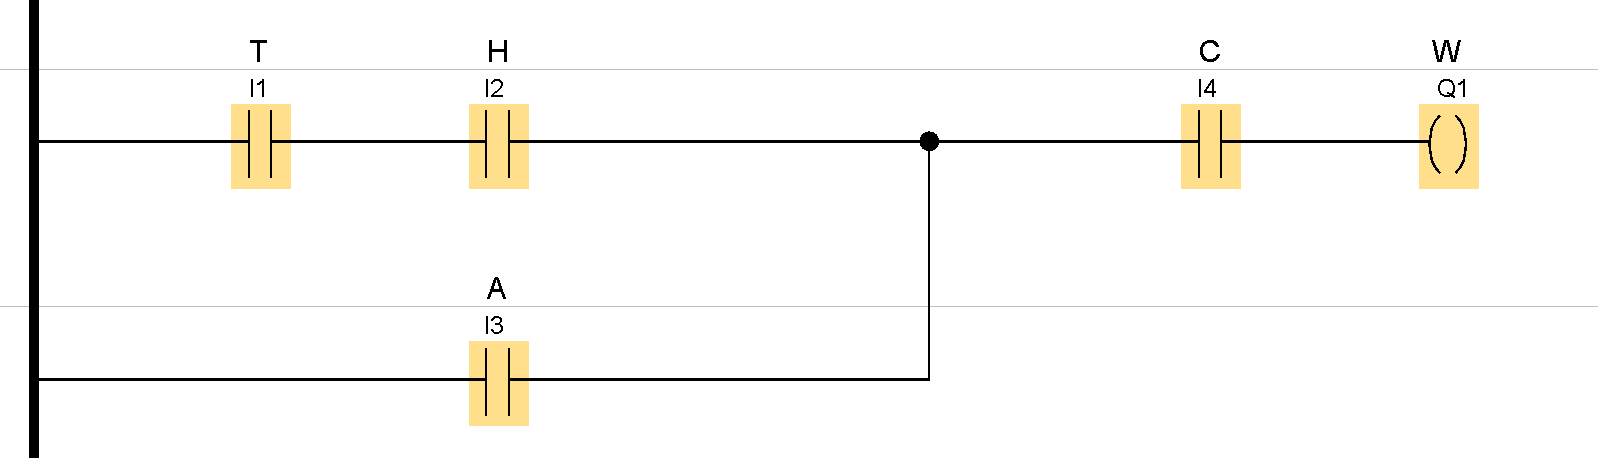
\includegraphics[width=0.92\textwidth]{rys/zad3/3_1_schemat.png}
    \caption{Drabinka zadania 3}
    \label{fig:z3-drabinka}
\end{figure}

Symulacja pokazuje trzy rzeczy, o które w tej funkcji chodzi. Przy przekroczonej temperaturze i wilgotności oraz przy zasilaniu wentylator pracuje, choć nikt nie wcisnął startu ręcznego (rys.~\ref{fig:z3-stany}a). Sam start ręczny przy zasilaniu też go załącza, przy $T = 0$ i $H = 0$ (rys.~\ref{fig:z3-stany}b). Gdy temperatura, wilgotność i start ręczny są jedynkami, a zasilania brakuje, Q1 zostaje zgaszone (rys.~\ref{fig:z3-stany}c).

\begin{figure}[H]
    \centering
    \begin{subfigure}{\textwidth}
        \centering
        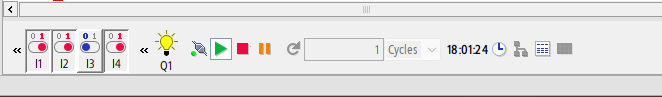
\includegraphics[width=0.72\textwidth]{rys/zad3/3_2_stan.png}
        \caption{$T = 1$, $H = 1$, $A = 0$, $C = 1$, Q1 załączone}
    \end{subfigure}

    \vspace{0.4em}
    \begin{subfigure}{\textwidth}
        \centering
        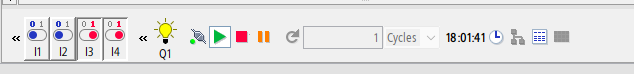
\includegraphics[width=0.72\textwidth]{rys/zad3/3_3_stan.png}
        \caption{$T = 0$, $H = 0$, $A = 1$, $C = 1$, Q1 załączone}
    \end{subfigure}

    \vspace{0.4em}
    \begin{subfigure}{\textwidth}
        \centering
        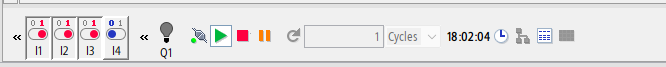
\includegraphics[width=0.72\textwidth]{rys/zad3/3_4_stan.png}
        \caption{$T = 1$, $H = 1$, $A = 1$, $C = 0$, Q1 zgaszone}
    \end{subfigure}
    \caption{Symulacja zadania 3}
    \label{fig:z3-stany}
\end{figure}
